\chapter{Využití Hjorthových deskriptorů na odhad TF a kvality signálů}
\label{ch:hjorth}
% Důvody použití Hjorthových deskriptorů pro odhad TF.
% - Metoda nevyžaduje identifikaci systolických vrcholů.
% Argumentace robustností vůči šumu a periodicitou PPG signálu.
% Hjorthovy parametry se běžně používají v EEG (např. pro klasifikaci stavů), ale pro TF z PPG je to méně časté - a tedy inovativní.
V této kapitole je popsán alternativní přístup k odhadu srdeční tepové frekvence (\acs{TF}) z fotopletysmografického signálu (\acs{PPG}), využívající Hjorthovy deskriptory (také označované jako Hjorthovy parametry).
Na rozdíl od standardních metod~\cite{ENIKÖ,Charlton2022,NeuroKit2}, které se opírají o detekci jednotlivých systolických vrcholů a případně výpočet \acs{IBI}, využívá tento přístup frekvenční vlastnosti analyzovaného signálu.
To je výhodou v případech, kdy je signál poškozen šumem, artefakty, nebo když je kladen důraz na výpočetní náročnost a rychlost algoritmu.

V podkapitole~\ref{sec:hjorth_kvalita} je popsán způsob využití Hjorthových deskriptorů pro hodnocení kvality signálu. % extend

Hjorthovy deskriptory představují trojici časových charakteristik, původně zavedených Hjorthem v roce 1970 pro kvantitativní popis elektroencefalografických (\acs{EEG}) signálů~\cite{Hjorth1973}.
Jedná se o parametry \textit{aktivita} (\(H_0\)), \textit{mobilita} (\(H_1\)) a \textit{komplexita} (\(H_2\)), které odrážejí střední výkon, střední frekvenci a šířku pásma.
Jejich výpočet vychází čistě z časové domény a nevyžaduje transformaci do frekvenční oblasti.

V oblasti zpracování \acs{PPG} signálů byly Hjorthovy parametry doposud využívány převážně pro hodnocení kvality signálu a detekci artefaktů~\cite{Peralta2017}. % some more references for quality
Právě proto je v naší práci navržen a realizován nový způsob odhadu \acs{TF} na základě Hjorthovy \textit{mobility} (\(H_1\)).
Tu počítáme na filtrovaných a čtyřnásobně autokorelovaných signálech.
Struktura navrženého algoritmu je znázorněna na Obr.~\ref{fig:hjorth_schemata}.

\begin{figure}[h]
	\centering
	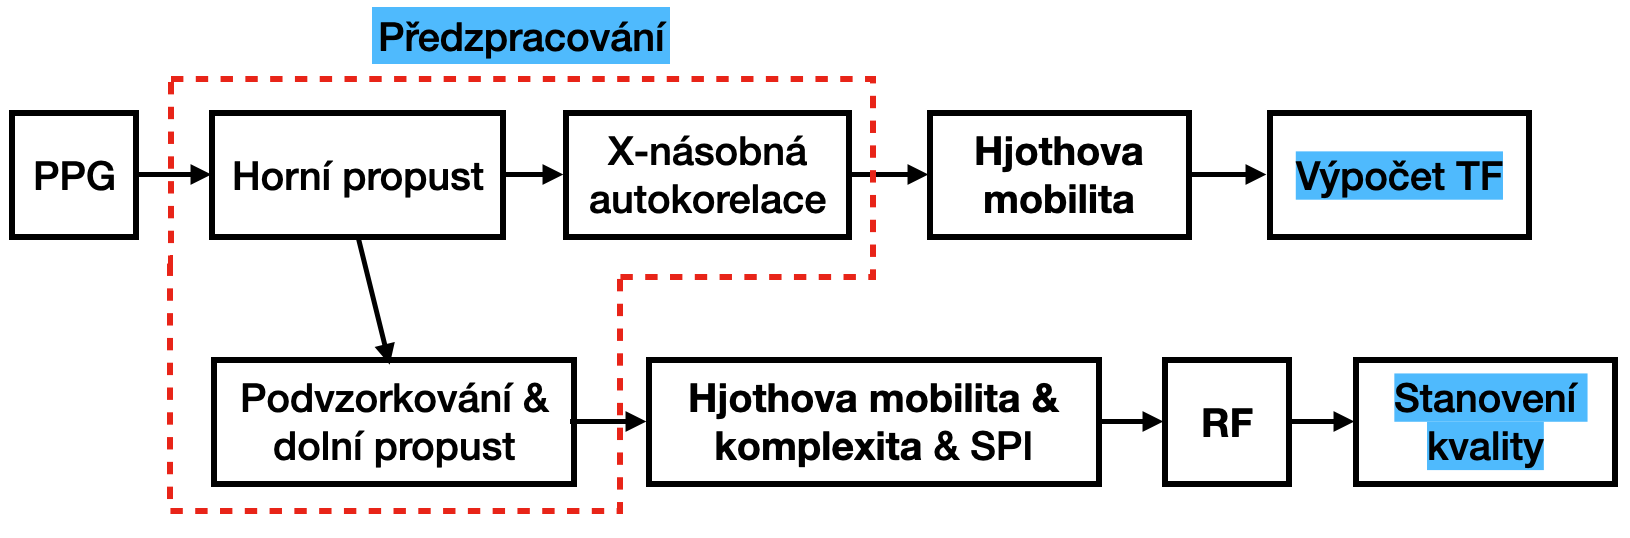
\includegraphics[width=1\textwidth]{./obrazky/hjorth_schema.png} % aktualizovat hodnocení kvality?
	\caption[Schéma našeho algorimu, který využívá Hjorthových deskriptorů]{Blokové schéma našeho využití Hjorthových deskriptorů.}
	\label{fig:hjorth_schemata}
\end{figure}

\section{Využití mobility pro odhad TF}
\label{sec:hjorth_mobilita_TF}
% Načtení signálu z databází probíhá stejně jako u \ref{sec:alg_load}
% Rozdělení signálů je více modulativní, než u \ref{sec:alg_split} pro CapnoBase můžeme použít celý signál nebo libovolný počet oken s maximální délkou odpovídající 10s signálu. Pro BUT PPG (10s signály) to není možné.

\subsection*{Zpracování signálu}
\label{sec:zpracovani}
% High-pass filtraci pro odstranění DC a respirační složky.
% Jak fungiuje autokorelace (4x) - cílem je zvýraznění periodické složky.
% Grafy autokorelace, původní signál, frekvenční spektrum obou signálů.
% KEEP IN MIND: Nepotlačují se frekvence, ale složky o vyšších/nižších frekvencích.
Hjorthovy deskriptory byly vypočítány z \acs{PPG} signálů, které byly nejprve předzpracovány ve dvou krocích.

Prvním krokem byla aplikace horní propusti s mezní frekvencí 0,5~Hz (odpovídající minimální \acs{TF}).
Cílem této filtrace bylo potlačit složky s nižšími frekvencemi, jako je stejnosměrná složka (\acs{DC}) a nebo respirační vliv.

Druhým kromem bylo aplikování čtyřnásobná autokorelace, čímž došlo k zvýraznění dominantní periodické struktury signálu a potlačení nepravidelných složek. % extend by explanation of autocorrelation

Porovnání filtrovaného a autokorelovaného signálu je znázorněno na Obr.~\ref{fig:hjorth_autocorr} společně s jejich frekvenčními charakteristikami.

\begin{figure}[t]
	\centering
	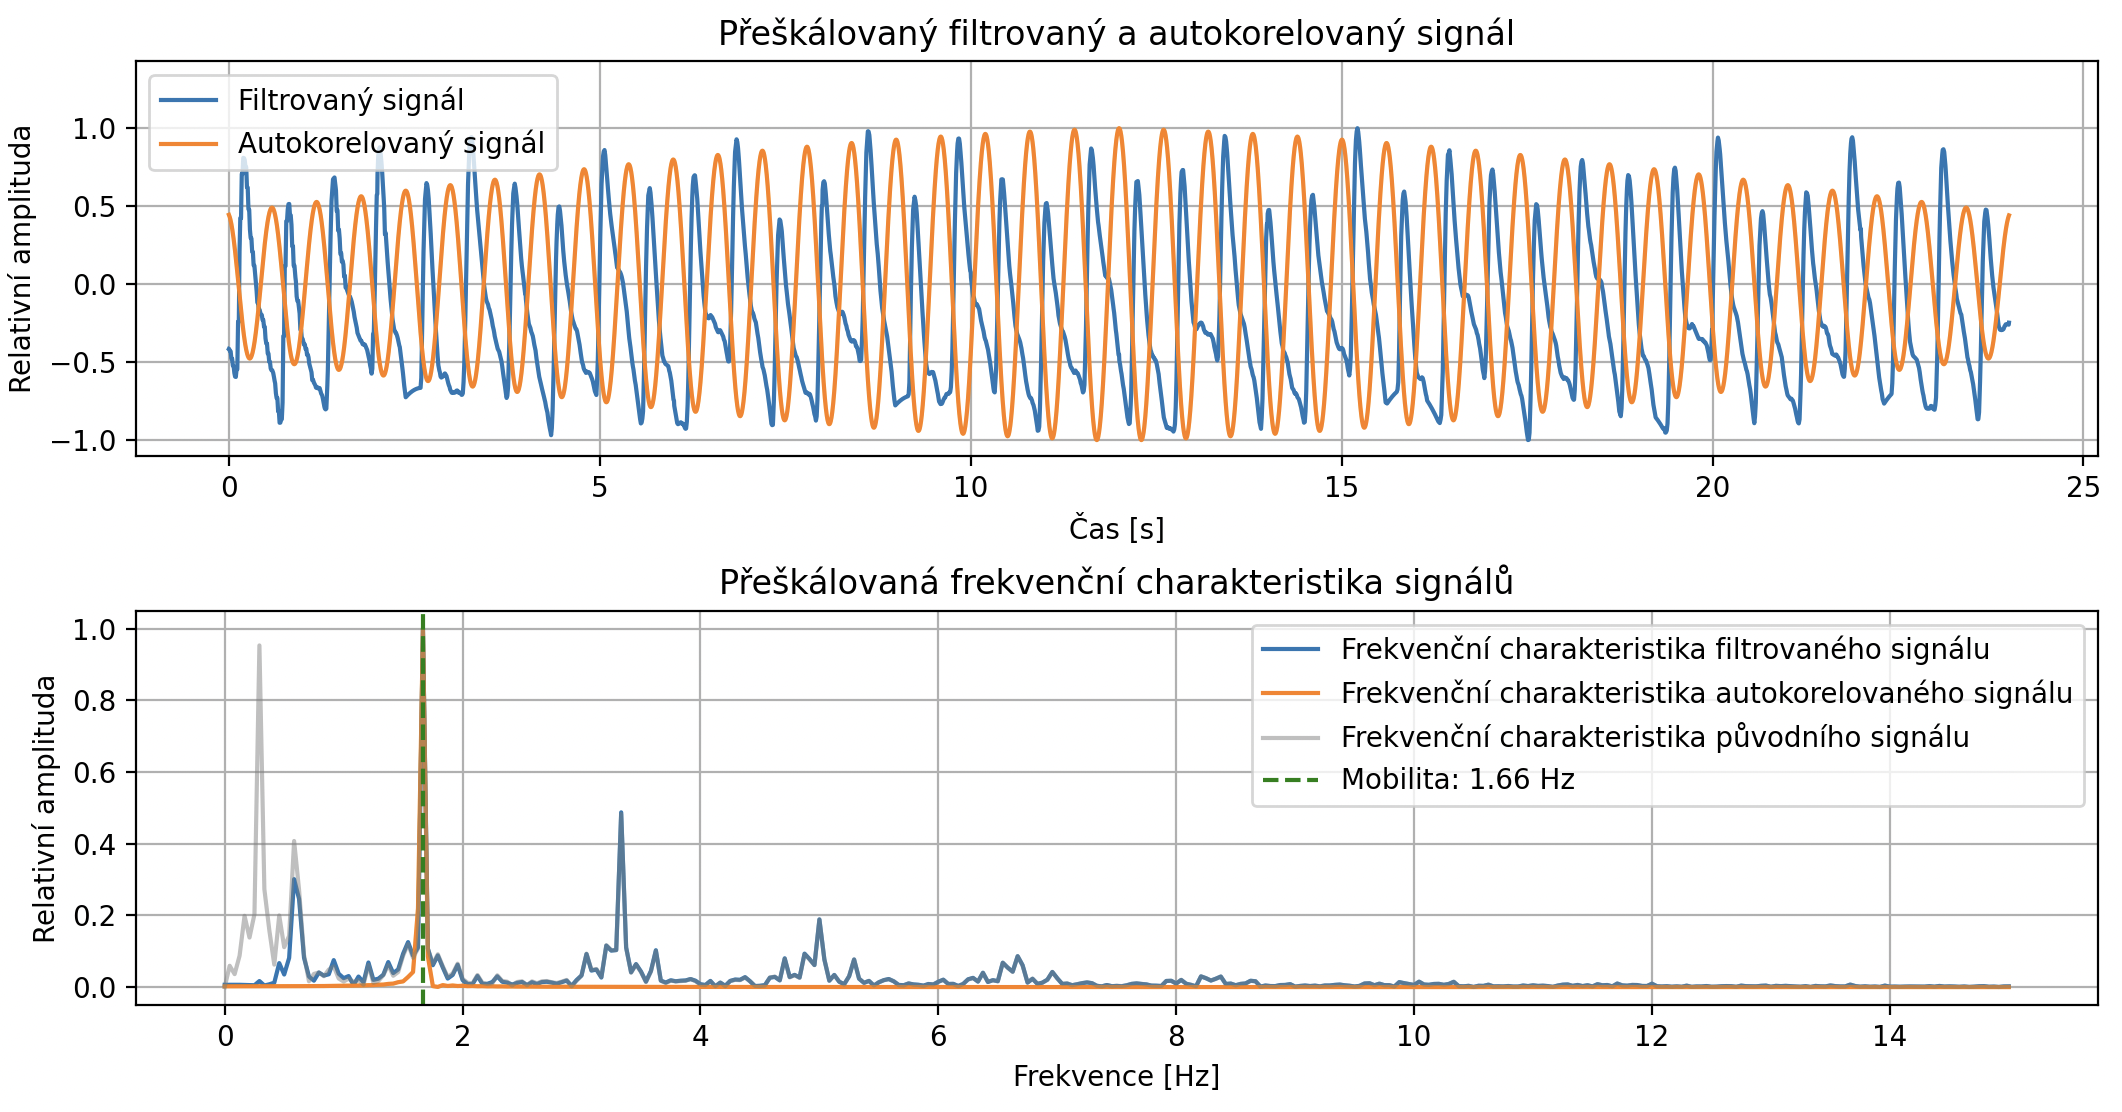
\includegraphics[width=1\textwidth]{./obrazky/hjorth_autocorr_freq.png}
	\caption[Porovnání filtrovaného a autokorelovaného signálu]{Porovnání filtrovaného a autokorelovaného signálu.}
	\label{fig:hjorth_autocorr}
\end{figure}

\subsection*{Výpočet TF z mobility}
\label{sec:TF_mobilita}
% Vysvětlení co znamenajá mobilita a jak se počítá -> vzorec.
% - Mobilita_autokor
% Jak se počítá TF z mobility - vzorec.


\section{Využití mobility a komplexity pro hodnocení kvality signálu}
\label{sec:hjorth_kvalita}
% Vysvětlení co znamenajá mobilita a komplexita a jak se počítají -> vzorec.
% - Mobilita_filtr a Komplexita_filtr
% Vysvětlit jak se počítá SPI
% Jaké prahy jsme nastavili pro hodnocení kvality signálu.